\documentclass{article}
\usepackage{ctex}
\usepackage{booktabs}
\usepackage{geometry}
\newgeometry{
    top=30mm, bottom=25mm, left=30mm, right=20mm,
    headsep=5mm
}
%页边距

\usepackage{titlesec} %自定义多级标题格式的宏包
\titleformat{\section}[block]{\LARGE\bfseries}{\arabic{section}}{1em}{}[]
\titleformat{\subsection}[block]{\Large\bfseries}{\arabic{section}.\arabic{subsection}}{1em}{}[]
\titleformat{\subsubsection}[block]{\normalsize\bfseries}{\arabic{subsection}-\alph{subsubsection}}{1em}{}[]
\titleformat{\paragraph}[block]{\small\bfseries}{[\arabic{paragraph}]}{1em}{}[]

\iffalse
\titleformat{command}[shape]%定义标题类型和标题样式,字体
{format}%定义标题格式:字号(大小),加粗,斜体
{label}%定义标题的标签,即标题的标号等
{sep}%定义标题和标号之间的水平距离
{before-code}%定义标题前的内容
[after-code]%定义标题后的内容
\fi

\usepackage{graphicx} %插入图片的宏包
\usepackage{float} %设置图片浮动位置的宏包
\usepackage{subfigure} %插入多图时用子图显示的宏包
\usepackage[hidelinks]{hyperref}

\begin{document}
\begin{titlepage}
    % 第二个()里的参数表示左移35pt,下移55pt
    \begin{picture}(0,0)(35,55)
        \includegraphics[width=90pt]{figure/buaamark.eps}
    \end{picture}
    \hfill

    \vskip 95bp
    \begin{center}
        \includegraphics[width=360bp]{figure/buaaname.eps}
        \vskip 45bp
        \centerline{\zihao{-0}\heiti 时间序列分析课程论文}
        ~~\\
        \vspace*{\stretch{4}}
        \begin{minipage}[h]{.8\textwidth}
            \centering{\heiti\zihao{2}时间序列分析课程论文}
        \end{minipage}
        \vskip 20bp
        \begin{minipage}[h]{.75\textwidth}
            \centering{\heiti\zihao{3}时间序列分析课程论文}
        \end{minipage}
        \vspace*{\stretch{3}}
        ~~\\
        {
        \zihao{-3}\heiti
        \begin{tabular}{cc}
            学~~~院~~~名~~~称~~ & \underline{~~~~学院~~~~} \\[.4ex]
            专~~~业~~~名~~~称~~ & \underline{~~~~专业~~~~} \\[.4ex]
            学~~~生~~~姓~~~名~~ & \underline{~~~李俊然~~~} \\[.4ex]
            指~~~导~~~教~~~师~~ & \underline{~~~123~~~~~}  \\
        \end{tabular}

        }
        \vskip 60bp
        \centerline{\heiti\zihao{-3}2021~~年~~5~~月~~23~~日}
    \end{center}
\end{titlepage}
\pagenumbering{gobble}
\newpage
\tableofcontents


\newpage
\pagenumbering{arabic}
\section{绪论}
\subsection{问题描述}
在现代,对于气象数据的预测对于某些商业活动非常重要,如何根据过去的气象数据对于未来的天气条件进行预测是一个值得研
究的问题
\subsection{数据来源}
数据来自于Kaggle,源自Weather Undergroud API。数据包含了2013年1月1日到2017年4月24日德里(Delhi)的每日平均气温、
湿度、风速、气压数据,本模型利用了温度进行时间序列分析。
\section{数据描述}
以下是训练数据的前几行

\begin{table}[htbp]
    \centering    
    \begin{tabular}{rrrrr}
        \multicolumn{1}{l}{date} & \multicolumn{1}{l}{meantemp} & \multicolumn{1}{l}{humidity} & \multicolumn{1}{l}{wind\_speed} & \multicolumn{1}{l}{meanpressure} \\
        \midrule
        2013/1/1                 & 10.00                        & 84.50                        & 0.00                            & 1015.67                          \\
        2013/1/2                 & 7.40                         & 92.00                        & 2.98                            & 1017.80                          \\
        2013/1/3                 & 7.17                         & 87.00                        & 4.63                            & 1018.67                          \\
        2013/1/4                 & 8.67                         & 71.33                        & 1.23                            & 1017.17                          \\
        2013/1/5                 & 6.00                         & 86.83                        & 3.70                            & 1016.50                          \\
        2013/1/6                 & 7.00                         & 82.80                        & 1.48                            & 1018.00                          \\
        2013/1/7                 & 7.00                         & 78.60                        & 6.30                            & 1020.00                          \\
        2013/1/8                 & 8.86                         & 63.71                        & 7.14                            & 1018.71                          \\
        2013/1/9                 & 14.00                        & 51.25                        & 12.50                           & 1017.00                          \\
        2013/1/10                & 11.00                        & 62.00                        & 7.40                            & 1015.67                          \\
        \bottomrule
    \end{tabular}%
    \label{data_head}%
    \caption{部分训练数据}
\end{table}%

建立模型只使用了每日平均温度数据,均值为25.51$^{\circ}$C,标准差为7.339416$^{\circ}$C,
其随时间变化的图形如下。

\begin{figure}[H]
    \centering % 图片居中
    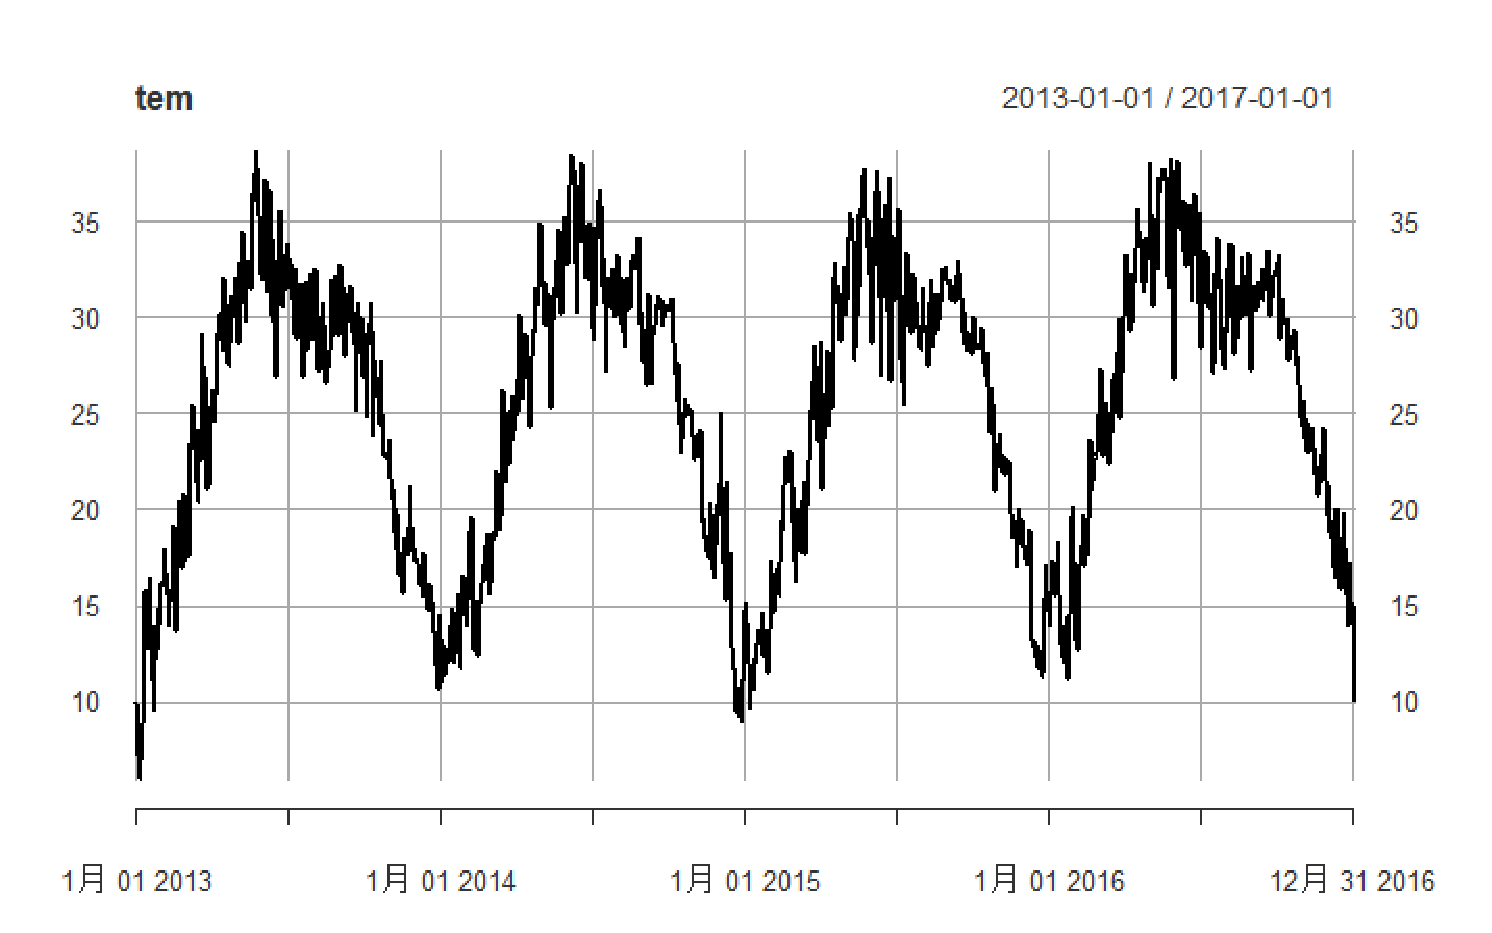
\includegraphics[width = 8.3cm]{figure/01.eps}
    \caption{气温时间序列图}
    \label{tem_seq}
\end{figure}

可以看到其呈现强烈的季节性趋势。

\section{模型构建}
考虑到平均气温存在季节性趋势,我们建立模型
$$X_t=(T_t-T_{t-1})-(T_{t-365}-T_{t-366})$$
其中$T_t$是第t期气温,$X_t$为进行了差分之后的新变量,接下来对于$X_t$进行时间序列分析。

\begin{figure}[H]
    \centering % 图片居中
    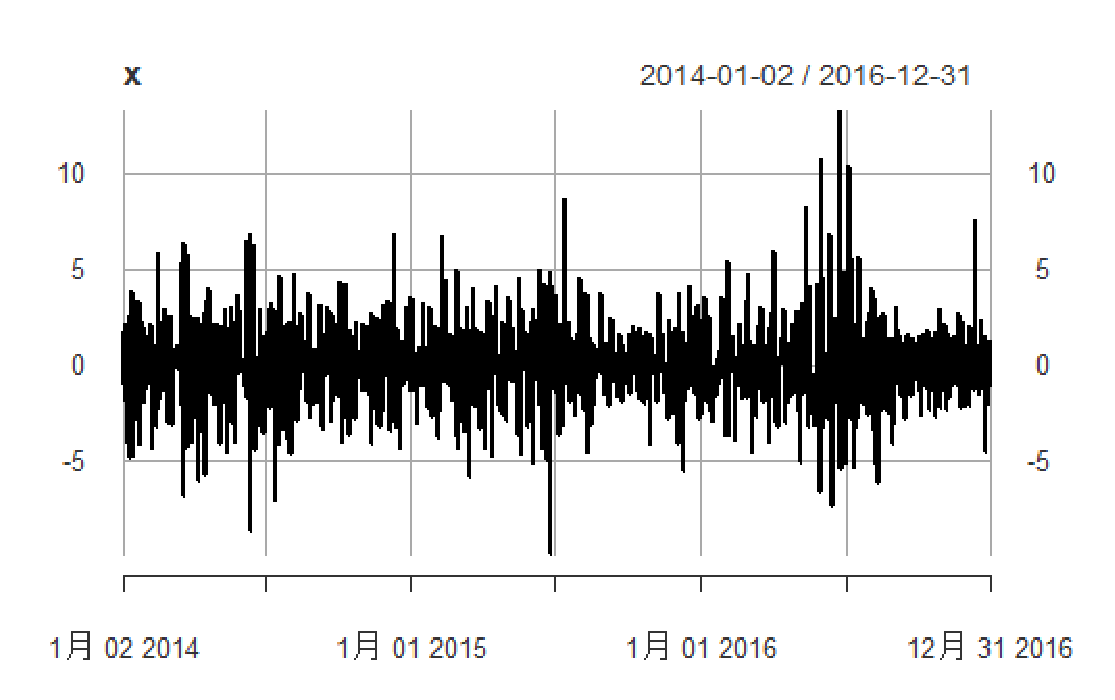
\includegraphics[width = 8.3cm]{figure/02.eps}
    \caption{X时间序列图}
    \label{x_seq}
\end{figure}
可以看到整体序列较为稳定,对其进行adf检验,得到的P-value为0.01,拒绝了存在单位根的原假设,
也就是说序列是平稳的,下一步进行ARAM建模。

\subsection{ARAM建模}

首先,自相关和偏自相关图如下

\begin{figure}[H]
    \centering  %图片全局居中
    \subfigure[ACF]{
    \label{ACF}
    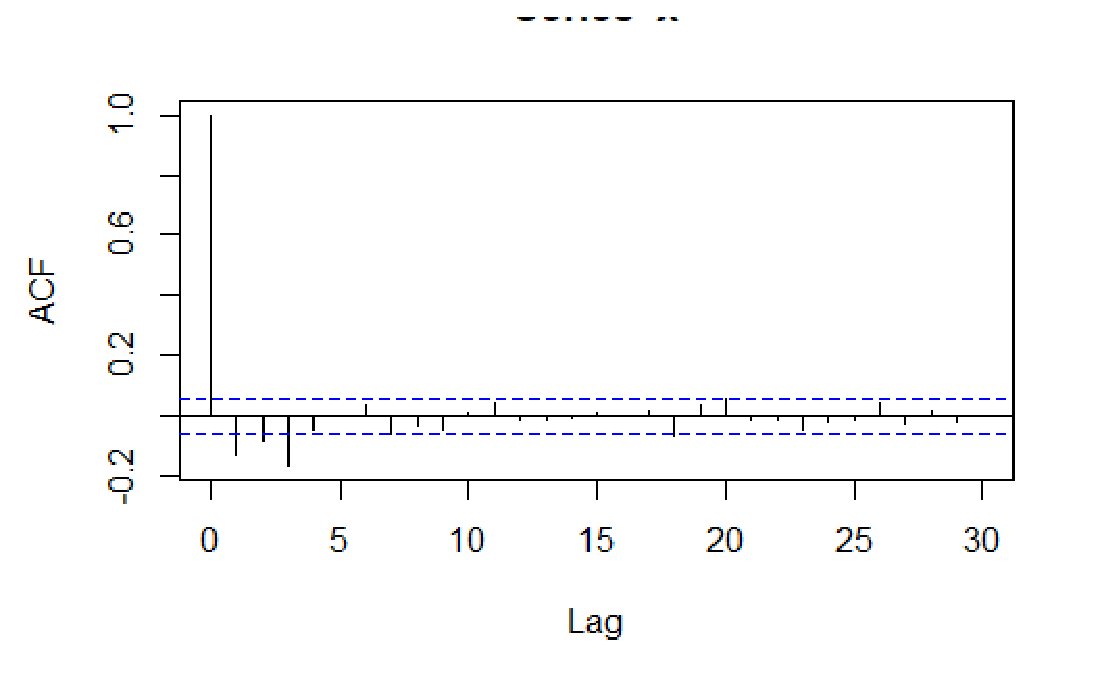
\includegraphics[width=0.45\textwidth]{03.eps}}
    \subfigure[PACF]{
    \label{PACF}
    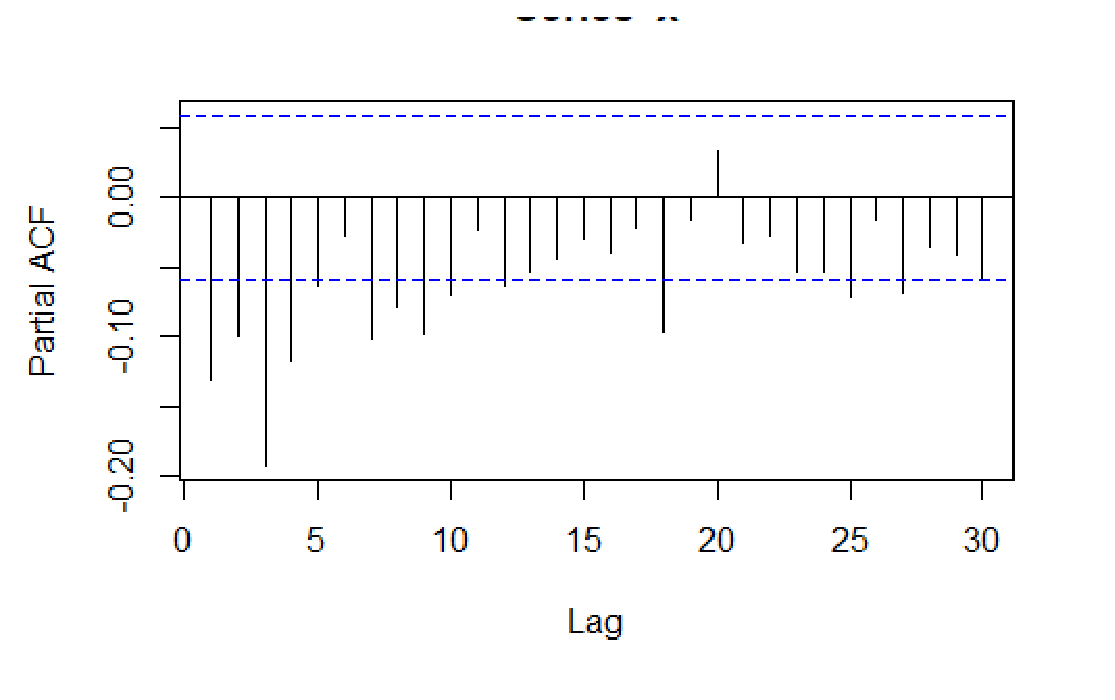
\includegraphics[width=0.45\textwidth]{04.eps}}
    \caption{自相关和偏自相关图}
    \label{ACF_PACF}
\end{figure}
由于ACF图和PACF图的截尾性不强,因此使用基于AIC信息量最小原则来识别模型阶数,
经过计算得到最佳模型为ARAM(1,2),此时AIC=4779.87,模型系数为
$$x_t=0.6977X_{t-1}-0.9674*a_{t-1}-0.0220*a_{t-2}$$
系数方差如下表

% Table generated by Excel2LaTeX from sheet 'Sheet1'
\begin{table}[htbp]
    \centering
    \caption{Add caption}
      \begin{tabular}{llll}
            & ar1   & ma1   & ma2 \\
  \cmidrule{2-4}    Coefficient & 0.6977 & -0.9674 & -0.022 \\
      s.e.  & 0.0332 & 0.0429 & 0.0406 \\
      \end{tabular}%
    \label{aram12}%
\end{table}%

对于残差,考虑是否存在条件异方差,对于残差序列进行了Arch检验,由于在PACF图中为5步截尾,
Arch检验步幅设置为5,在显著性水平为0.05的条件下拒接了原假设,认为序列存在Arch效应,
因此接下来对模型进行改进,建立ARAM+Arch模型

\begin{figure}[H]
    \centering % 图片居中
    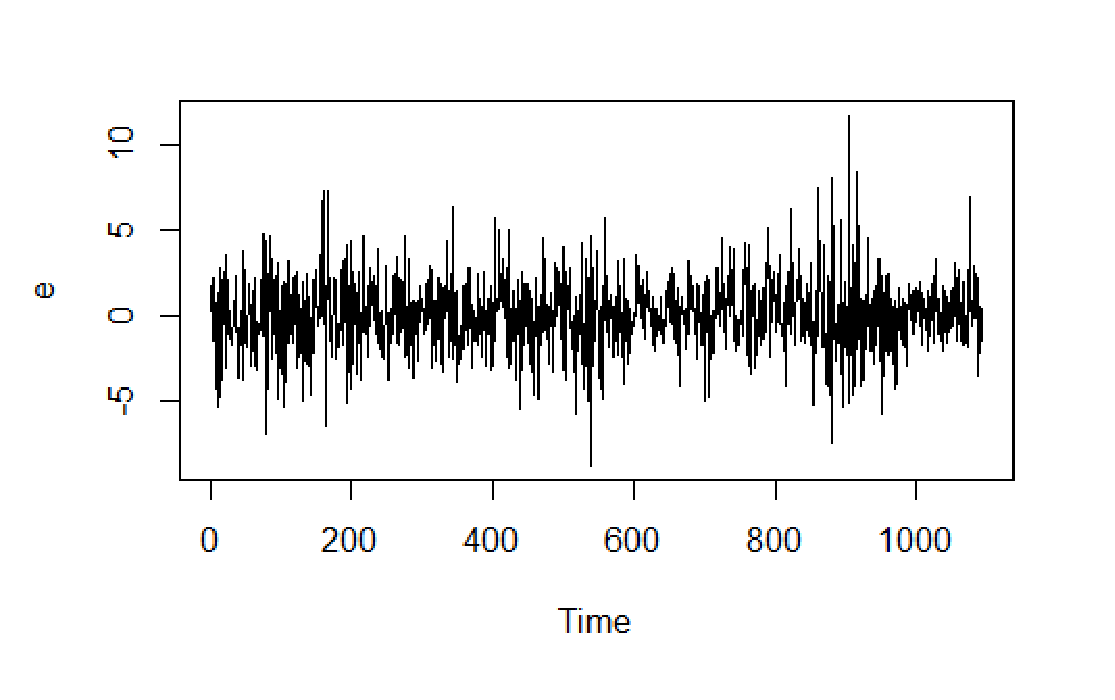
\includegraphics[width = 8.3cm]{figure/05.eps}
    \caption{残差时间序列图}
    \label{e_seq}
\end{figure}

\subsection{ARAM+Arch模型}
首先,我们建立了arma(1, 2)+garch(5,0)模型,使用R中fGarch包进行了模型参数求解,
得到的结果如下

% Table generated by Excel2LaTeX from sheet '新建文本文档'
\begin{table}[htbp]
    \centering
    \caption{Add caption}
      \begin{tabular}{lllll}
            & Estimate & Std.Error & tvalue & Pr(>|t|) \\
  \cmidrule{2-5}    mu    & 2.40E-04 & 3.13E-03 & 0.077 & 0.938778 \\
      ar1   & 6.59E-01 & 3.61E-02 & 18.24 & <2e-16 \\
      ma1   & -8.93E-01 & 4.60E-02 & -19.391 & <2e-16 \\
      ma2   & -5.79E-02 & 4.20E-02 & -1.376 & 0.168779 \\
      omega & 3.11E+00 & 2.80E-01 & 11.097 & <2e-16 \\
      alpha1 & 1.34E-01 & 3.65E-02 & 3.68  & 0.000233 \\
      alpha2 & 5.80E-02 & 3.57E-02 & 1.624 & 0.104384 \\
      alpha3 & 1.00E-08 & 4.97E-02 & 0     & 1 \\
      alpha4 & 6.83E-02 & 3.23E-02 & 2.116 & 0.034354 \\
      alpha5 & 7.51E-02 & 3.46E-02 & 2.175 & 0.029623 \\
      \bottomrule
      \end{tabular}%
    \label{aram+garch1}%
\end{table}%

去掉模型中不显著的参数(显著性水平为0.05),模型简化为arma(1, 1)+garch(1,0),重新进行参数求解,
得到的结果如下

% Table generated by Excel2LaTeX from sheet '1'
\begin{table}[htbp]
    \centering
    \caption{Add caption}
      \begin{tabular}{lllll}
            & Estimate & Std.Error & tvalue & Pr(>|t|) \\
  \cmidrule{2-5}    mu    & 0.0001924 & 0.0014865 & 0.129 & 0.897029 \\
      ar1   & 0.7030944 & 0.024831 & 28.315 & <2e-16 \\
      ma1   & -0.9772436 & 0.0069917 & -139.772 & <2e-16 \\
      omega & 3.9265142 & 0.2121147 & 18.511 & <2e-16 \\
      alpha1 & 0.1456684 & 0.0391164 & 3.724 & 0.000196 \\
      \bottomrule
      \end{tabular}%
    \label{aram+garch2}%
\end{table}%

可以看到模型中参数都是显著的



\section{模型预测检验}
21
\end{document}